{\actuality}

%%%
% Роторные насосы являются сложной системой и находят применение в различных областях (еще сложнее когда качают кровь)
% Необходима идентификация для определения параметров насоса
%%%

В настоящее время аппараты вспомогательного кровообращения (АВК) успешно применяются при лечении различных форм сердечной недостаточности. Основным элементом АВК является имплантируемый роторный насос крови (РНК), который является сложной технической системой, помогающей поддерживать кровообращение в сердечно-сосудистой системе. Основным параметром РНК является скорость вращения ротора, от которой зависит степень поддержки кровообращения.

% Сердечная недостаточность (СН) является тяжелым, прогрессирующим заболеванием, которое характеризуется неспособностью сердца перекачивать кровь в объеме, достаточном для обеспечения метаболических потребностей организма. На данный момент наиболее эффективным способом лечения тяжелых форм сердечной недостаточности является трансплантация сердца. 
% 
% Вследствие дефицита донорских сердец для трансплантации в последние десять лет активное развитие получили аппараты вспомогательного кровообращения (АВК), используемые для лечения пациентов с различными формами СН. Основным компонентом данных аппаратов является имплантируемый роторный насос крови (РНК), который благодаря непрерывному вращению ротора помогает поддерживать необходимый уровень кровообращения. 

Одним из ключевых направлений развития технологии вспомогательного кровообращения, позволяющим повысить эффективность лечения сердечной недостаточности, является управление имплантируемым РНК. В литературе предложено множество способов управления РНК с использованием скорости вращения ротора в качестве управляемой переменной. Для управления имплантируемыми роторными насосами крови необходима их идентификация, то есть построение математической модели по результатам экспериментальных исследований. Изучению проблемы идентификации сложных технических систем посвящен целый ряд фундаментальных исследований российских и зарубежных авторов: Д. Гроппа, Л. Льюнга, С. А. Акулова и А. А. Федотова, В. М. Трояновского и др. \cite{identification_usa, identification_ljung, biotech_basics, trojan}. %результатам экспериментального исследования. 

В настоящее время решением проблемы идентификации насосов, в том числе имплантируемых роторных насосов крови, занимается большое количество исследователей. Значительный вклад в исследования и практическое применение полученных результатов был внесен такими учеными, как Г. П. Иткин, К. Н. Дозоров, Ю. В. Солодянников, А. Б. Тмур, F. Moscato, T. Pirbodaghi и др. \cite{vest_2015, dozorov_2009, solod_1994, tmur_2014, Moscato_2009, Pirbodaghi_2017}.% Работы данных исследователей в большинстве случаев направлены на построение математических моделей точно аппроксимирующих экспериментальные данные и не анализируют эффективность управления имплантируемыми роторными насосами крови. 

% В то же время не существует универсального способа идентификации имплантируемых РНК, что обусловлено их многообразием, сложным устройством, зависимостью производительности насосов от состояния сердечно-сосудистой системы и, как следствие, строгим требованием учитывать взаимодействие насосов с сердечно-сосудистой системой. %Вместе с этим, работы по идентификации имплантируемых РНК, как правило, направлены на повышение точности аппроксимации исходных экспериментальных данных математической моделью, и не проводят исследования эффективности управления имплантируемыми роторными насосами крови. % рассматривают эффективность управления имплантируемыми роторными насосами крови.

Идентификация имплантируемых роторных насосов крови остается сложной задачей и в настоящее время не существует универсального и общепринятого способа идентификации. Это обусловлено многообразием и сложным устройством роторных насосов крови, зависимостью производительности насосов от состояния сердечно-сосудистой системы и, как следствие, строгим требованием учитывать взаимодействие насосов с сердечно-сосудистой системой. Исследования по идентификации роторных насосов крови направлены на построение математических моделей точно аппроксимирующих экспериментальные данные, при этом необходимым является исследование эффективности идентификации для управления роторными насосами крови с использованием построенных математических моделей.

%В то же время не существует общепринятого и универсального алгоритма идентификации, что обусловлено сложностью описания работы имплантируемого роторного насоса и непрерывным взаимодействием сердечно-сосудистой системы и насоса, которые образуют сложную систему. 

Таким образом, актуальной является задача идентификации имплантируемых роторных насосов крови с использованием универсального алгоритма, что требует структурной идентификации, которая заключается в представлении объекта управления в виде математической модели с определением ее структуры, и параметрической идентификации, которая заключается в определении числовых значений коэффициентов математической модели согласно экспериментальным данным, с последующим исследованием и оценкой эффективности идентификации для управления имплантируемыми роторными насосами крови в аппаратах вспомогательного кровообращения.

% Таким образом, для повышения эффективности лечения пациентов с сердечной недостаточностью посредством аппаратов вспомогательного кровообращения еобходима разработка подходов к регулированию работы РНК, обеспечивающих возможность диагностики состояния сердечно-сосудистой системы и автоматизированное регулирование параметров АВК с целью поддержания определенных уровней производительности РНК или состояний в сердечно-сосудистой системе.
% 
%  Настоящая работа посвящена разработке методов и алгоритмов управления работой имплантируемого роторного насоса крови для аппаратов вспомогательного кровообращения. Предполагается, что они позволят разрешить указанные проблемы и предотвратить физиологические нарушения при экплуатации АВК, что в долгосрочной перспективе должно привести к улучшению результатов лечения. 
% 
% -----------------------------------------------------------------------------------------------------------------------------------
% -----------------------------------------------------------------------------------------------------------------------------------

\textbf{Объектом исследования} являются имплантируемые роторные насосы крови в аппаратах вспомогательного кровообращения.

\textbf{Предметом исследования} являются методы и алгоритмы структурно-параметрической идентификации имплантируемых роторных насосов крови в аппаратах вспомогательного кровообращения.

\textbf{Проблемная ситуация, сложившаяся в области объекта исследований}, определяется тем, что идентификация имплантируемых роторных насосов крови в аппаратах вспомогательного кровообращения является сложной и актуальной научно-технической задачей, которая требует разработки методов и алгоритмов структурной и параметрической идентификации, обеспечивающих высокую эффективность управления имплантируемыми роторными насосами крови в аппаратах вспомогательного кровообращения. 

Общая схема поддержки кровообращения с помощью АВК приведена на рисунке \ref{img:system_links}. Взаимодействие АВК с телом пациента может быть представлено взаимодействием РНК, крови, сосудов и сердца; основными параметрами данной системы являются расход насоса $Q(t)$ и перепад давления в насосе $H(t)$, которые зависят от скорости вращения ротора насоса $\omega(t)$. % отражает состояние сердечно-сосудистой системы и взаимосвязан с $Q(t)$ и $\omega(t)$. 

\begin{figure}[ht]
  \begin{minipage}[ht]{0.43\linewidth}
    \center{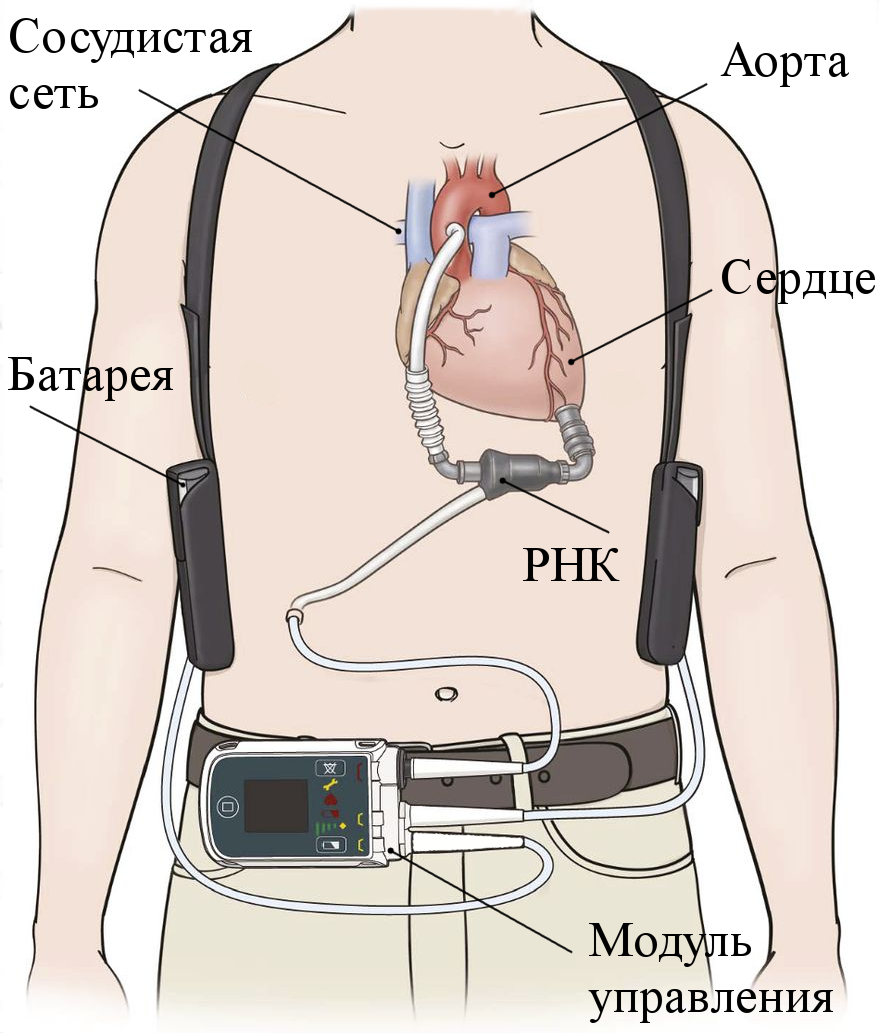
\includegraphics [scale=0.9] {../images/vad_system}}
  \end{minipage}
  \hfill
  \begin{minipage}[ht]{0.55\linewidth}
    \center{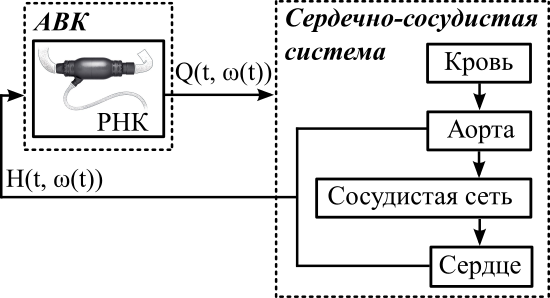
\includegraphics [scale=1.85] {../images/system_links}}
  \end{minipage}
  \caption{Представление аппарата вспомогательного кровообращения (АВК) в виде системы, образованной роторным насосом крови (РНК) и сердечно-сосудистой системой; $Q(t)$ -- расход насоса, $\omega(t)$ -- скорость вращения ротора насоса, $H(t)$ -- перепад давления в насосе, $t$ -- время}
  \label{img:system_links}  

\begin{tikzpicture}[node distance=1cm, overlay]  
\tikzstyle{arrow} = [thick,->,>=stealth]
\draw [arrow] (6.4, 6.3) |- (7.6, 6.3);
\draw [arrow] (7.4, 5.6) |- (6.2, 5.6);
\end{tikzpicture} 

\end{figure}

% В левой части рисунка \ref{img:system_links} представлена схема взаимодействия АВК и тела пациента; в правой части -- процесс взаимодействия АВК и сердечно-сосудистой системы при помощи РНК. При этом расход насоса $Q(t)$ определяется скоростью вращения ротора $\omega(t)$ и взаимосвязан с параметрами сердечно-сосудистой системы.

% При этом также возникает необходимость разработки методов и алгоритмов идентификации таких систем.

 \aim\ диссертационной работы является разработка и исследование способов структурно-параметрической идентификации имплантируемых роторных насосов крови для повышения эффективности идентификации и управления имплантируемыми роторными насосами крови в аппаратах вспомогательного кровообращения.

%разработка и исследование алгоритма идентификации для управления имплантируемым роторным насосом крови в аппаратах вспомогательного кровообращения.

% идентификация и управление имплантируемым роторным насосом крови в аппаратах вспомогательного кровообращения.
% \newpage
В~соответствии с целью диссертационной работы поставлены следующие {\tasks}:
\begin{enumerate}
  \item Разработка математической модели идентификации имплантируемого роторного насоса крови на основе расходно-напорных характеристик.
  \item Разработка математической модели сердечно-сосудистой системы с учетом имплантации роторного насоса крови.
  \item Исследование взаимодействия имплантируемого роторного насоса крови и сердечно-сосудистой системы методами математического моделирования и анализ результатов исследования с целью повышения эффективности идентификации и управления имплантируемым роторным насосом крови.
  \item Исследование взаимодействия имплантируемого роторного насоса крови и сердечно-сосудистой системы с использованием экспериментальных данных для роторных насосов крови Спутник с целью верификации результатов математического моделирования.
%   \item Разработать алгоритм идентификации имплантируемого роторного насоса крови на основе расходно-напорных характеристик, полученных в результате экспериментального исследования имплантируемых роторных насосов крови и опубликованных в литературе.
%   \item Исследовать разработанный алгоритм идентификации имплантируемого роторного насоса крови с использованием математической модели сердечно-сосудистой системы. % возможности алгоритма для управления имплантируемым роторным насосом крови с помощью моделирования взаимодействия  роторного насоса и сердечно-сосудистой системы в условиях сердечной недостаточности. % можно описать раздельно или переформулировать
%   \item Исследовать разработанный алгоритм идентификации с использованием результатов экспериментального исследования имплантируемых роторных насосов крови <<Спутник>> в испытательном гидродинамическом стенде.
%   \item Разработать способ управления имплантируемым роторным насосом крови на основе результатов исследования алгоритма идентификации. 
\end{enumerate}

% -----------------------------------------------------------------------------------------------------------------------------------
% -----------------------------------------------------------------------------------------------------------------------------------
%\newpage
\novelty
\begin{enumerate}
  % что нового в разработке, исследовании и управлении?
  \item Разработан алгоритм структурно-параметрической идентификации, который позволяет построить математическую модель в соответствии с критериями оценки эффективности идентификации для управления имплантируемыми роторными насосами крови. \\На основе построенной математической модели разработан способ управления имплантируемым роторным насосом крови, направленный на поддержание заданного уровня расхода насоса и предотвращение следующих нежелательных режимов работы насоса: обратное течение через насос, полная разгрузка желудочка сердца и коллапс желудочка сердца.
  \item Предложены следующие критерии, которые позволяют оценить эффективность идентификации для управления имплантируемыми роторными насосами крови: точность оценки расхода насоса и точность определения перехода между режимами работы насоса. \\С использованием алгоритма структурно-параметрической идентификации и в соответствии с предложенными критериями оценки эффективности идентификации построены математические модели имплантируемых роторных насосов крови Спутник.
  \item В результате комплексного исследования взаимодействия имплантируемого роторного насоса крови и сердечно-сосудистой системы на основе математической модели идентификации разработан метод определения следующих режимов работы имплантируемого роторного насоса крови: обратное течение через насос, частичная и полная разгрузка желудочка сердца, и коллапс желудочка сердца.
\end{enumerate}

% -----------------------------------------------------------------------------------------------------------------------------------
% -----------------------------------------------------------------------------------------------------------------------------------

\influence\ 
\begin{enumerate}
 \item Разработанные программные средства использованы при моделировании взаимодействия имплантируемого роторного насоса крови и сердечно-сосудистой системы и теоретическом исследовании имплантируемых роторных насосов крови Спутник. 
 \item Разработанный алгоритм структурно-параметрической идентификации может быть использован для управления имплантируемыми роторными насосами крови при проведении экспериментальных исследований в испытательных гидродинамических стендах. % напиши конкретно на ком и на чем
\end{enumerate}

% -----------------------------------------------------------------------------------------------------------------------------------
% -----------------------------------------------------------------------------------------------------------------------------------

\underline{\textbf{Личный вклад автора.}}

Автор принимал активное и непосредственное участие в выполнении всех работ, которые легли в основу диссертации.

\defpositions

\begin{enumerate}
  % с требуемой точностью % обеспечивает следующие возможности для управления: оценка расхода насоса и определение режимов работы насоса. %\vskip5pt
  %\item Разработан алгоритм идентификации, который позволяет повысить эффективность управления имплантируемым роторным насосом крови в аппаратах вспомогательного кровообращения.
 % \item Разработанный метод определения режимов работы имплантируемого роторного насоса крови позволяет определять следующие переходы между режимами работы насоса, что подтверждается результатами моделирования и исследования с использованием экспериментальных данных для роторных насосов крови Спутник: обратное течение через насос, частичная и полная разгрузка желудочка сердца, и коллапс желудочка сердца. %, что подтверждается результатами моделирования и исследования с использованием экспериментальных данных.
 \item Предложены критерии, которые позволяют оценить эффективность идентификации для управления имплантируемыми роторными насосами крови в аппаратах вспомогательного кровообращения.
  \item Разработанный алгоритм структурно-параметрической идентификации позволяет построить математические модели имплантируемых роторных насосов крови в соответствии с критериями оценки эффективности идентификации.
  \item Построенные математические модели имплантируемых роторных насосов крови позволяют определить переходы между следующими режимами работы насоса: обратное течение через насос, частичная и полная разгрузка желудочка сердца, и коллапс желудочка сердца.
  \item Разработанный способ управления имплантируемым роторным насосом крови позволяет поддерживать заданный уровень расхода насоса и предотвращать следующие нежелательные режимы работы насоса: обратное течение через насос, полная разгрузка желудочка сердца и коллапс желудочка сердца. 
 %, что позволяет повысить эффективность управления насосом в аппаратах вспомогательного кровообращения.
  %\item Разработанная модель идентификации имплантируемого роторного насоса крови позволяет описать расходно-напорные характеристики с требуемым уровнем точности. 
\end{enumerate}

% \begin{enumerate}
%   \item Разработанная математическая модель имплантируемого роторного насоса крови позволяет учесть влияние вязкости и инерции жидкости на расходно-напорные характеристики роторного насоса крови.
%   \item Разработанный метод определения режимов работы насоса позволяет с высокой точностью определить режимы работы насоса посредством анализа динамики течения жидкости через насос с помощью математической модели роторного насоса крови. %исследования на математической модели сердечно-сосудистой системы и результатами верификации с использованием данных экспериментального исследования. 
%   \item Разработанный алгоритм управления работой имплантируемого роторного насоса крови обеспечивает соответствие основным требованиям к управлению работой имплантируемого роторного насоса крови для аппаратов вспомогательного кровообращения.
%   \item Предложенный алгоритм разработки математической модели имплантируемого роторного насоса крови на основе результатов экспериментального исследования роторного насоса крови позволяет обеспечить высокую точность оценки расхода насоса и определения режимов работы насоса.
% \end{enumerate}


% -----------------------------------------------------------------------------------------------------------------------------------
% -----------------------------------------------------------------------------------------------------------------------------------

\methodology\ % Основными методами исследования в диссертационной работе являются методы математического моделирования и оптимизации. %Экспериментальное исследование выполнено \textit{in vitro} в испытательном гидродинамическом стенде. % программных библиотек
%Обоснованность результатов моделирования подтверждена данными экспериментальных исследований на гидродинамическом стенде.

% пиши конкретно: экспериментальное исследование чего? методы исследования можно отразить в задачах работы

Методами исследования диссертационной работы являются методы системного анализа и математического моделирования. 

%Обработка и анализ данных выполнены с использованием языка программирования Python.
%Идентификация имплантируемых роторных насосов крови проведена с использованием алгоритмов оптимизации Левенберга-Марквардта и дифференциальной эволюции. 

% -----------------------------------------------------------------------------------------------------------------------------------
% -----------------------------------------------------------------------------------------------------------------------------------

\reliability\ полученных результатов обусловлена корректностью поставленных задач, комплексным характером проведенных исследований и согласием полученных результатов с литературными данными. %литературными данными и результатами экспериментального исследования. 

%использованием апробированных методов моделирования
%использованием проверенных подходов к моделированию динамики кровообращения

% -----------------------------------------------------------------------------------------------------------------------------------
% -----------------------------------------------------------------------------------------------------------------------------------

\probation\
Основные результаты диссертационной работы были представлены на следующих конференциях: % докладывались

\begin{itemize}
 \item 44th Annual ESAO and 7th IFAO Congress (г. Вена, Австрия, 2017),
 \item 2nd International Symposium <<Physics, Engineering and Technologies for Biomedicine>> (г. Москва, 2017),
 \item 20-23-я всероссийская конференция <<Микроэлектроника и информатика>> (г. Москва, 2013 -- 2016),
 \item 61-62nd ASAIO Annual Conference (г. Чикаго, США, 2015; г. Сан-Франциско, США, 2016),
 \item 24th Congress of the International Society for Rotary Blood Pumps (г. Мито, Япония, 2016),
 \item X-XI German-Russian Conference on Biomedical Engineering (г. Санкт-Петербург, 2014; г. Ахен, Германия, 2015),
 \item 42th Annual ESAO Congress (г. Лёвен, Бельгия, 2015),
 \item 37th Annual International Conference of the IEEE Engineering in Medicine and Biology Society (г. Милан, Италия, 2015),
 \item 16-я научно-техническая конференция <<МедТех>> (о. Кефалония, Греция, 2014),
 \item 11-я международная конференция <<Физика и радиоэлектроника в медицине и экологии>> (г. Суздаль, 2014),
 \item 6-я Троицкая конференция <<Медицинская физика и инновации в медицине>> (г. Троицк, 2014).
\end{itemize}

\implement\
Результаты диссертационной работы получены в рамках следующих проектов и исследований:

\begin{itemize}
 \item проект Российского научного фонда № 14-39-00044 <<Разработка адаптивной системы вспомогательного кровообращения с целью персонализации лечения острой формы сердечной недостаточности>> (2014 -- 2016 гг.) по приоритетному направлению <<Проведение фундаментальных научных исследований и поисковых научных исследований вновь создаваемыми научной организацией и вузом совместными научными лабораториями>>,
 \item прикладные научные исследования в рамках ФЦП <<Исследования и разработки по приоритетным направлениям развития научно-технологического комплекса России на 2014 – 2020 годы>> по теме <<Разработка аппарата длительного механического замещения функции сердца>> (RFMEFI57814X0057) (2014 -- 2016 гг.),
 \item прикладные научные исследования и экспериментальные разработки в рамках ФЦП <<Исследования и разработки по приоритетным направлениям развития научно-технологического комплекса России на 2014 – 2020 годы>> по теме <<Миниатюризация имплантируемых насосов крови для их применения в педиатрической кардиохирургии>> (RFMEFI58115X0014) (2015 -- 2017 гг.).
\end{itemize}

Результаты работы внедрены в учебный процесс института биомедицинских систем Национального исследовательского университета <<МИЭТ>> в рамках дисциплины <<Биомедицинская инженерия искусственных органов>> для магистров, обучающихся по направлению 12.04.04 <<Биотехнические системы и технологии>>.

%Российского научного фонда и Министерства образования и науки РФ в рамках ФЦП <<Исследования и разработки по приоритетным направлениям развития научно-технологического комплекса России на 2014 – 2020 годы>>.

%Результаты диссертационной работы использованы при реализации следующих проектов кафедры биомедицинских систем Национального исследовательского университета «МИЭТ»: 

%Исследования поддержаны Министерством образования и науки РФ в рамках ФЦП <<Исследования и разработки по приоритетным направлениям развития научно-технологического комплекса России на 2014 – 2020 годы>> по теме <<Разработка аппарата длительного механического замещения функции сердца>> (RFMEFI57814X0057) на 2014 -- 2016 г. и теме <<Миниатюризация имплантируемых насосов крови для их применения в педиатрической кардиохирургии>> (RFMEFI58115X0014) на 2015 -- 2017 г., и Российским научным фондом по теме <<Разработка адаптивной системы вспомогательного кровообращения с целью персонализации лечения острой формы сердечной недостаточности>> (проект № 14-39-00044) на 2014 -- 2016 г.

%\contribution\ Автор принимал активное участие \ldots № 14.578.21.0057 (RFMEFI57814X0057)  № 14.581.21.0014 (RFMEFI58115X0014) 

% -----------------------------------------------------------------------------------------------------------------------------------
% -----------------------------------------------------------------------------------------------------------------------------------

\publications\ Результаты по теме диссертации изложены в 29 научных работах, из них 11 опубликованы в рецензируемых научных изданиях, входящих в перечень Высшей аттестационной комиссии при Министерстве образования и науки Российской Федерации и в международную реферативную базу данных Scopus, 18 -- в тезисах докладов всероссийских и международных конференций. % По теме диссертации опубликована 21 научная работа, из них 8 изданы в журналах, 
